\documentclass[a4paper,review,12pt,authoryear]{elsarticle}

\usepackage{natbib}
\usepackage{amsfonts,amsmath,bbm,bm,xcolor,booktabs,hyperref,amsthm}
\usepackage[ruled]{algorithm2e}
\usepackage{geometry}
\usepackage{subfig}
\geometry{a4paper,scale=0.8}
\usepackage{setspace}
\setstretch{1.5}
\let\code=\texttt
\let\proglang=\textsf
\setcounter{MaxMatrixCols}{20}
\usepackage{soul}
\hypersetup{
  colorlinks=true,
  linkcolor=blue,
  citecolor=blue,
  urlcolor=blue}

% ADDING LINENUMBERS FOR REVIEWING:
\usepackage{lineno}

\newcommand{\bY}{\mathbf{Y}}
\newcommand{\bpi}{\bm{\pi}}
\newcommand\independent{\protect\mathpalette{\protect\independenT}{\perp}}
\def\independenT#1#2{\mathrel{\rlap{$#1#2$}\mkern2mu{#1#2}}}


\theoremstyle{definition}
\newtheorem{definition}{Definition}[section]

\begin{document}

\begin{frontmatter}

  \title{Discrete forecast reconciliation}

  \author[label1]{Bohan Zhang}
  \address[label1]{School of Economics and Management, Beihang University, Beijing, China}
  \author[label2]{Anastasios Panagiotelis}

  \author[label1]{Yanfei Kang\corref{cor1}}
  \ead{yanfeikang@buaa.edu.cn}
  \cortext[cor1]{Corresponding author.}
  \address[label2]{The University of Sydney Business School, NSW 2006, Australia}

  \begin{abstract}

    While forecast reconciliation has seen great success for real valued data, the method has not yet been comprehensively extended to the discrete case. This paper defines and develops a formal discrete forecast reconciliation framework based on optimising scoring rules using quadratic programming. The proposed framework produces coherent joint probabilistic forecasts for count hierarchical time series.
    Two discrete reconciliation algorithms are proposed and compared to generalisations of the top-down and bottom-up approaches to count data. Two simulation experiments and two empirical examples are conducted to validate that the proposed reconciliation algorithms improve forecast accuracy. The empirical applications are to forecast criminal offences in Washington D.C. and sales of product units in M5 dataset. Compared to benchmarks, the proposed framework shows superior performance in both simulations and empirical studies.

  \end{abstract}

  \begin{keyword}
  Forecasting \sep
  Hierarchical time series \sep
  Count data \sep
  Brier score \sep
  Quadratic programming.
  \end{keyword}

\end{frontmatter}

%\clearpage
\newpage
\linenumbers

\section{Introduction}

Non-negative time series with discrete values, particularly those with low counts, commonly arise in various fields.
Examples include intermittent demand in the retail industry (\citealp{kourentzesElucidateStructureIntermittent2021}), occurrences of ``black swan'' events during a period (\citealp{nikolopoulosWeNeedTalk2020}) and incidents of violent crime within a specific block.
Count hierarchical time series (HTS) are naturally constructed when decisions in multiple cross-sectional or temporal aggregation levels must be made.
In the past decades, hierarchical forecasting has attracted significant attention from the forecasting community, yielding many innovative approaches and applications (see \citealp{athanasopoulosForecastReconciliationReview2023} and references wherein).
However, most existing hierarchical approaches are intrinsically designed for continuous-valued time series and can not be directly applied to discrete-valued data.
This paper aims to fill this gap by proposing a discrete reconciliation approach to produce coherent forecasts for low-count HTS.

The core objective of hierarchical forecasting is to produce \textit{coherent} forecasts,
in the sense that the point forecast for a parent series should equal the sum of the point forecasts for the associated child series. Historically, this was accomplished by producing forecasts at one level
and then aggregating or disaggregating them into other levels (\citealp{fliednerHierarchicalForecastingIssues2001}).
An alternative approach, also known as \textit{forecast reconciliation}, proposed by \cite{hyndmanOptimalCombinationForecasts2011} and further explored by \cite{wickramasuriyaOptimalForecastReconciliation2019}, \cite{panagiotelisForecastReconciliationGeometric2021}, and others involves
first generating independent \textit{base} forecasts for each time series,
which are then ``optimally'' reconciled to produce coherent forecasts. These state-of-art approaches have shown the ability to produce coherent and potentially more accurate forecasts.

Concerning forecasting count time series, it is natural to produce distributional forecasts rather than solely point forecasts.
The predictive distribution describes the full uncertainty of future events for optimal decision-making (\citealp{gneitingProbabilisticForecasting2014}).
Forecast reconciliation has already been extended to probabilistic forecasting.
Earlier approaches created coherent probabilistic forecasts by reconciling samples drawn from base forecasts, resulting in a coherent empirical distribution.
\cite{jeonProbabilisticForecastReconciliation2019} propose a method that draws samples from the independently modelled predictive distributions and constructs base forecasts using stacking, ranking, or permutation techniques before reconciling them with the reconciliation matrix obtained through cross-validation.
In contrast, \cite{bentaiebHierarchicalProbabilisticForecasting2020} construct coherent samples through the bottom-up approach,
where the dependence among bottom time series is restored using empirical copula modelling.
Recently, \cite{panagiotelisProbabilisticForecastReconciliation2022} introduce a formal framework for probabilistic reconciliation based on the concept of probabilistic coherence.
They also propose an efficient algorithm to compute reconciliation weights by optimising proper scoring rules.


Despite the rapid development of reconciliation approaches, most existing approaches can not be easily adapted to count time series.
Regarding point forecasts, the reconciliation approaches yield non-integer forecasts because they project base forecasts from an incoherent real space onto a coherent real subspace (\citealp{panagiotelisForecastReconciliationGeometric2021}).
While rounding is a practical way to deal with non-integer forecasts, the rounded forecasts may not be coherent anymore.
In terms of distributional forecasts, it can even be more challenging to discretise the distributions while maintaining the probabilistic coherence.
Therefore, it makes more sense to develop a hierarchical forecasting approach that handles discrete distributions directly.

Another motivation of our study lies in forecast combination, which serves as one of the crucial elements contributing to superior performance of forecast reconciliation (\citealp{hollymanUnderstandingForecastReconciliation2021}).
In forecast reconciliation, every reconciled forecast is a weighted combination of all base forecasts that can incorporate external information using arbitrary forecasting methods.
More importantly, the reconciliation process avoids the requirement for complex models that simultaneously capture hierarchical constraints, external information, and serial dependence.
Given these advantages, the reconciliation framework is a reasonable choice for forecasting count HTSs while allowing existing univariate count forecasting approaches in the literature to be employed effectively.

To the best of our knowledge, existing literature on count HTS forecasting is limited and not tailored for low-count time series.
\cite{coraniProbabilisticReconciliationCount2022} propose a novel reconciliation approach that conditions base probabilistic forecasts of the most disaggregated series on base forecasts of aggregated series.
The reconciled forecasts are derived by generalising Bayes’ rule and Monte Carlo sampling.
\cite{zambonEfficientProbabilisticReconciliation2022} further extend this idea to accommodate both count time series and real-valued time series.
Although this innovative approach yields coherent probabilistic forecasts,
the conditional manner employed can fail to account for the dependence structure within hierarchical time series.
Incorporating correlation necessitates base predictive distributions that are obtained through multivariate base models, which, notwithstanding advances in methods such as copulas, remain challenging.

In this paper, we seek to address the hierarchical forecasting problem for discrete-valued time series, particularly focusing on low-count time series.
Firstly, we introduce the notion of ``coherence'' for hierarchical counts,
bearing a resemblance to the probabilistic coherence proposed by \cite{panagiotelisProbabilisticForecastReconciliation2022}.
Secondly, we utilise these concepts to establish a formal reconciliation framework for count HTSs, which generally reconciles the forecasts by assigning probability from incoherent to coherent domain points.
Thirdly, we adopt the Brier score as a metric for evaluating forecasts and present a reconciliation algorithm that optimises this metric.
We also demonstrate how this algorithm can be solved through quadratic programming, and to speed up the computation, we develop a second stepwise algorithm.
Fourthly, two simulation experiments are performed to verify the applicability in both temporal and cross-sectional settings.
Lastly, we conduct two empirical experiments using real data. The first experiment analyses a crime dataset with a temporal hierarchy, and the other employs cross-sectional sales data in the M5 dataset.

The remainder of this paper is organised as follows.
Section \ref{sec:coherence} presents the notation and the concept of coherence for count HTSs.
Section \ref{sec:method} details the proposed discrete reconciliation framework based on optimising the Brier score through Quadratic programming. The stepwise algorithm is also introduced in this section.
Section \ref{sec:simulation} performs two simulation experiments in cross-sectional and temporal settings, and two empirical experiments are conducted in Section \ref{sec:application}.
Then, Section \ref{sec:discussion} presents discussions and thoughts on future research. 
Finally, Section \ref{sec:conclusion} concludes the paper.



\section{Coherence of probabilistic hierarchical count forecasts}

\label{sec:coherence}

% \subsection{Preliminaries}

Consider an $n$-vector $\bY=\left(Y_1,Y_2,\ldots,Y_n\right)'$ of discrete random variables.
We partition $\bY$ so that the first $m$ elements are \textit{basis} variables and the remaining $(n-m)$ elements are \textit{determined} variables.
The determined variables are some deterministic functions of the basis variables. Usually, the basis variables are the bottom-level or most disaggregated data, while the determined variables are obtained from aggregating the bottom-level variables differently.
Each element of $\bY$ has a finite domain given by $\mathcal{D}(Y_i)=\left\{0, 1,2,3,\dots,D_i\right\}$, where $i = 1, 2, \dots, n$.

\subsection{Discrete coherence}\label{sec:domains}

Defining coherence in the discrete setting first requires definitions of three sets upon which predictive distributions can be defined. The \textit{complete domain} of $\bY$ is given by
\[
\hat{\mathcal D}(\bY)=\prod\limits_{i=1}^n\hat{\mathcal D}(Y_i)=\left\{0, 1,2,\dots,D_1\right\}\times\left\{0,1,2,\dots,D_2\right\}\times\dots\times\left\{0,1,2,\dots,D_n\right\},
\]
where products are Cartesian products taken over sets, i.e. any possible vector where each element corresponds to a possible discrete value of a single variable.
The cardinality of the complete domain is $|\hat{\mathcal D}(\bY)|=\prod\limits_{i=1}^{n} (D_i+1)$, which is denoted by $q$.
The complete domain is analogous to $\mathbb{R}^n$ in the continuous case.

The \textit{coherent domain} of $\bY$, denoted as $\tilde{\mathcal D}(\bY)$, is given by a subset of $\hat{\mathcal D}(\bY)$, for which aggregation constraints hold.
It has cardinality $|\tilde{\mathcal D}(\bY)|=\prod\limits_{i=1}^{m} (D_i+1)$, which we denote as $r$.
The coherent domain is analogous to the coherent subspace $\mathfrak{s}$ in the continuous case (\citealp{panagiotelisProbabilisticForecastReconciliation2022}). The \textit{incoherent domain} $\bar{\mathcal D}(\bY)$ is defined as the set difference between the complete domain and incoherent domain, i.e. the set of points for which the aggregation constraints do not hold.

  \subsubsection*{\textbf{Example}.}
  \label{sec:example}

  Let $Y_1$ and $Y_2$ be binary variables and $Y_3=Y_1+Y_2$. In this case, the domain of each variable is
  \[
    \mathcal{D}(Y_1)=\left\{0,1\right\},\quad
    \mathcal{D}(Y_2)=\left\{0,1\right\},\quad
    \mathcal{D}(Y_3)=\left\{0,1,2\right\}.
  \]
  The complete domain is
  \begin{equation}
  \begin{aligned}
  \hat{\mathcal D}(\bY)=&\left\{\mathbf{(0,0,0)'},(0,1,0)',(1,0,0)',(1,1,0)',\right.\\
  &\left.(0,0,1)',\mathbf{(0,1,1)'},\mathbf{(1,0,1)'},(1,1,1)',\right.\\
  &\left.(0,0,2)',(0,1,2)',(1,0,2)',\mathbf{(1,1,2)'}\right\}\,,
  \end{aligned}
  \label{eq:incoherent}
  \end{equation}
  and the coherent domain consists of those points for which $y_1+y_2=y_3$, highlighted in \textbf{bold} in Equation~\eqref{eq:incoherent}. Thus, the coherent domain is
  \[
      \tilde{\mathcal D}(\bY)=\left\{(0,0,0)',(0,1,1)',(1,0,1)',(1,1,2)'\right\}\,,
  \]
  while the incoherent domain $\bar{\mathcal D}(\bY)$ is the set of points for which the aggregation constraints do not hold, i.e.
    \[
  \bar{\mathcal D}(\bY)=\left\{(0,1,0)',(1,0,0)',(1,1,0)',(0,0,1)',
  (1,1,1)',(0,0,2)',(0,1,2)',(1,0,2)'
  \right\}\,,
  \]
  
  \begin{definition}[Discrete coherence]
  
  A discrete coherent distribution has the property $Pr(\mathbf{Y}=\bm{y})=0, \forall \bm{y}\in \bar{\mathcal D}(\bY)$. Any distribution not meeting this condition is an incoherent distribution.

  \end{definition}

  \subsection{Coherency of predictive distribution for discrete-valued HTS}

  \label{sec:coherent_df}

  Assuming we aim to make a probabilistic $h$-step ahead forecast for $\bY$ at time $t$, we represent the resulting predictive distribution using a mapping function $\hat{\mathcal{H}}$ and a probability vector $\hat{\bpi}^{t+h|t}$, where each element corresponds to the probability of one discrete point in the complete domain.
  Two notational conventions are used for the elements of $\hat{\bpi}^{t+h|t}$.
  First, $\hat{\pi}_j^{t+h|t}$ denotes the $j^{th}$ element of $\hat{\bpi}^{t+h|t}$;
  second, $\hat{\pi}_{(y_1 y_2 \dots y_n)}^{t+h|t}$ denotes a specific element that corresponds to the forecast probability that $\bY$ takes on a value $(y_1,y_2,\dots,y_n)'$. These two conventions are linked by the function $\hat{\mathcal{H}}:{1,2,\dots,q}\rightarrow\hat{\mathcal{D}}(\bY)$, which maps each index $j$ to a configuration of values that $\bY$ can take.
  Using the small example in Section~\ref{sec:domains}, $\hat{\pi}_1^{t+h|t}=\hat{\pi}_{(000)}^{t+h|t}$, $\hat{\pi}_2^{t+h|t}=\hat{\pi}_{(010)}^{t+h|t}$, etc., and $\hat{\mathcal{H}}(1)=(0,0,0)'$, $\hat{\mathcal{H}}(2)=(0,1,0)'$, etc. Since this vector representation uniquely characterises a probability mass function, `probability vectors', `pmfs' and `distribution' will be used interchangeably throughout the rest of the paper.

  The predictive distribution is incoherent provided there exists some $\hat{\pi}^{t+h|t}_j\neq 0$ for which $\hat{\mathcal{H}}(j)\notin\tilde{\mathcal{D}}(\bY)$, i.e., non-zero probabilities are assigned to some points for which the aggregation constraints do not hold.
  This situation usually occurs in practice when probabilistic forecasts are generated independently for each variable, and the joint forecast is then constructed assuming independence.
  Such forecasts will generally be incoherent.
  For instance, in the simple example provided, if we suppose $Pr(Y_1=0)=0.2$,~$Pr(Y_2=1)=0.1$,~$Pr(Y_3=0)=0.05$, then under independence assumption we have $Pr(Y_1=0,Y_2=1,Y_3=0)=0.2\times0.1\times0.05=0.001$, which assigns non-zero probability to an incoherent point.

  On the other hand, a coherent probabilistic forecast can be defined using an $r$-vector $\tilde{\bpi}^{t+h|t}$ where each element corresponds to the probability of one point in the coherent domain.
  The notation $\tilde{\pi}_k^{t+h|t}$ represents the $k^{th}$ element of $\tilde{\bpi}^{t+h|t}$ and the notation $\tilde{\pi}_{(y_1 y_2 \dots y_n)}^{t+h|t}$ denotes a specific element of this vector that corresponds to the forecast probability that $\bY$ takes on a coherent value $(y_1,y_2,\dots,y_n)'$.
  The analogue to $\hat{\mathcal{H}}(j)$ is a function  $\tilde{\mathcal{H}}:{1,2,\dots,r}\rightarrow\tilde{\mathcal{D}}(\bY)$, which maps each index $k$ to a coherent configuration of values that $\bY$ can take.
  Using the small example in the previous section $\tilde{\pi}_1^{t+h|t}=\tilde{\pi}_{(000)}^{t+h|t}$, $\tilde{\pi}_2^{t+h|t}=\tilde{\pi}_{(011)}^{t+h|t}$, etc., and $\tilde{\mathcal{H}}(1)=(0,0,0)'$, $\tilde{\mathcal{H}}(2)=(0,1,1)'$, etc.

  \subsubsection*{\textbf{Example}.}

  Consider the earlier example in Section~\ref{sec:domains}, with binary $y_1$ and $y_2$ and $y_1+y_2=y_3$. The incoherent probabilistic forecast is given by
  \[
    \hat{\bpi}^{t+h|t}= \left[
      \hat{\pi}^{t+h|t}_{(000)}, ~
       \hat{\pi}^{t+h|t}_{(010)},~
       \hat{\pi}^{t+h|t}_{(100)},~
       \hat{\pi}^{t+h|t}_{(110)},~
       \hat{\pi}^{t+h|t}_{(001)},~
       \hat{\pi}^{t+h|t}_{(011)},~
       \hat{\pi}^{t+h|t}_{(101)},~
       \hat{\pi}^{t+h|t}_{(111)},~
       \hat{\pi}^{t+h|t}_{(002)},~
       \hat{\pi}^{t+h|t}_{(012)},~
       \hat{\pi}^{t+h|t}_{(102)},~
       \hat{\pi}^{t+h|t}_{(112)}
       \right]',
  \]
  where the notation $\hat{\pi}^{t+h|t}_{1}$ can be used instead of $\hat{\pi}^{t+h|t}_{(000)}$, and $\hat{\pi}^{t+h|t}_{2}$ can be used instead of $\hat{\pi}^{t+h|t}_{(010)}$, etc. Also, the function $\hat{\mathcal{H}}$ is defined so that $\hat{\mathcal{H}}(1)=(0,0,0)'$, $\hat{\mathcal{H}}(2)=(0,1,0)'$, etc.

  The coherent probabilistic forecast is given by
  \[
  \tilde{\bpi}^{t+h|t}=\left[
  \tilde{\pi}^{t+h|t}_{(000)},
  \tilde{\pi}^{t+h|t}_{(011)},
  \tilde{\pi}^{t+h|t}_{(101)},
  \tilde{\pi}^{t+h|t}_{(112)}
  \right]',\]
  where the notation $\tilde{\pi}^{t+h|t}_{1}$ can be used instead of $\tilde{\pi}^{t+h|t}_{(000)}$, and $\tilde{\pi}^{t+h|t}_{2}$ can be used instead of $\tilde{\pi}^{t+h|t}_{(011)}$, etc. Also, the function $\tilde{\mathcal{H}}$ is defined so that $\tilde{\mathcal{H}}(1)=(0,0,0)'$, $\tilde{\mathcal{H}}(2)=(0,1,1)'$, etc. Note that the ordering of the probabilities and the functions $\hat{\mathcal{H}}$ and $\tilde{\mathcal{H}}$ are not unique, which does not affect the proposed algorithms.

\section{Method}
\label{sec:method}

This section introduces a formal framework for discrete forecast reconciliation based on the discrete coherence defined in Section~\ref{sec:coherence}.
We then present an algorithm that optimises the Brier Score to find the optimal reconciliation matrix in Section~\ref{sec:algorithm} and Section~\ref{sec:algorithm1}.
To address the issue of dimensionality, we further propose a stepwise reconciliation algorithm that decomposes the hierarchy in Section~\ref{sec:algorithm2}.
Additionally, Section~\ref{sec:bottomup} extends the classical bottom-up and top-down approaches to the discrete case and demonstrates how they can be incorporated into our framework.

    \subsection{The discrete reconciliation framework}

    Loosely speaking, the discrete reconciliation framework constructs the coherent distribution by assigning mass from incoherent points to coherent points in the predictive distribution.
    Let $\tilde{\bpi} = \psi(\hat{\bpi})$ with the superscript $t+h|t$ dropped for convenience, where $\psi:[0,1]^q \rightarrow [0,1]^r$ is a reconciliation function that maps mass from the incoherent joint pmf to a coherent one.
    This framework is analogous to that described in \cite{panagiotelisProbabilisticForecastReconciliation2022}, where an incoherent probability measure on $\mathbb{R}^n$ is mapped onto the coherent subspace $\mathfrak{s}$.

    In this paper, we focus on the linear reconciliation function given by
    \begin{equation}
      \label{eq:framework}
    \tilde{\bpi}=\bm{A}\hat{\bpi},
    \end{equation}
    where $\tilde{\bpi}$ is obtained by multiplying the $r \times q$ matrix of reconciliation weights $\bm{A}$ with the incoherent probability vector $\hat{\bpi}$. Letting $a_{kj}$ be the element in row $k$ and column $j$ of $\bm{A}$, this is equivalent to
    \[
      \tilde{\pi}_k=\sum\limits_{j=1}^q a_{kj}\hat{{\pi}}_j
    \]
    for all $k = 1, 2, \dots, r$  and  $j = 1, 2, \dots, q$.
    Each $a_{kj}$ represents how much probability is shifted from the possibly incoherent point $\hat{\mathcal{H}}(j)$ to the coherent point $\tilde{\mathcal{H}}(k)$ (or from element $j$ in $\hat{\bpi}$ to element $k$ in $\tilde{\bpi}$). Note that $a_{kj}$ must meet the following constraints
    \begin{align*}
    0\leq a_{kj} \leq 1 , ~ \forall k, j, ~ \textrm{and} ~
    \sum\limits_{k=1}^r a_{kj} = 1 , ~ \forall j.
    \end{align*}
    The first constraint guarantees that the elements of $\tilde{\bpi}$ are between 0 and 1, while the second constraint guarantees that the elements of $\tilde{\bpi}$ sum to 1.
    Moreover, they imply that every point in the incoherent domain has its probability proportionally distributed among all points within the coherent domain.
    This process resembles the assignment problem commonly encountered in operational research.

    \subsection{Score optimal reconciliation}
    \label{sec:algorithm}

    Before introducing the objective function used to learn $\bm{A}$, we first introduce the evaluation of the reconciled distribution.
    Scoring rules $S(.,.)$ are commonly used for this purpose in probabilistic forecasting.
    These rules assign a numerical score based on the predictive distribution and the actual outcome, allowing for an optimisation procedure.
    An essential property for scoring rules is propriety. A scoring rule is said to be strictly proper if $\text{E}_Q[S(Q, \mathbf{y})] \leq \text{E}_Q[S(P, \mathbf{y})]$ with equality if and only if $P=Q$, where $P$ is any predictive distribution, $Q$ is the true distribution and $\mathbf{y}$ is an outcome.
    Alternative strictly proper scoring rules that can be used to evaluate discrete distributions include the Brier Score, spherical Score and logarithmic Score (see \citealp{gneitingStrictlyProperScoring2007} for more details).
    The Brier Score was initially proposed by \cite{brier1950verification}, and it has the following formulation:
    \[
      \text{BS}(\bpi, \mathbf{z}) = \sum_{k=1}^{O}(z_k - \pi_k)^2,
    \] where $\bpi$ is defined similarly as in Section~\ref{sec:coherent_df}.
    $k\in \{1,\dots,O\}$ is the index that can be mapped into the potential outcomes of an event through link function $\mathcal{H}$. $\mathbf{z}$ is the vectorization of the observation $\mathbf{y}$ with $z_k = 1$ if $\mathcal{H}(k) = \mathbf{y}$ and otherwise $0$.
    We choose the Brier score instead of other strictly scoring rules because it can seamlessly fit into our framework by formulating an objective function that can be solved through quadratic programming.

    Assume that $\hat{\bpi}^{t+h|t}$ are found for $t\in\mathcal{T}_{\textrm{window}}$, where $\mathcal{T}_{\textrm{window}}$ is an expanding window (\citealp{hyndmanForecastingPrinciplesPractice2021}).
    Figure~\ref{fig:rollingwindow} depicts the behaviour of the expanding window, where the training data always begins at the same origin, one observation is added to the training data for each window, and forecasts are made $h$ steps ahead. This process continues until the last observation is included in the forecast horizon.
    \begin{figure}
    \centering
    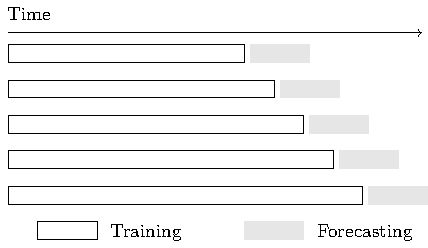
\includegraphics[width=0.5\textwidth]{figures/rolling_window.pdf}
    \caption{\label{fig:rollingwindow} Diagram of expanding window strategy.}
    \end{figure}
    Also, let $\mathbf{z}^{t+h}$ be an $r$-vector with element $z_k^{t+h}=1$ if $\tilde{\mathcal{H}}(k)=\bm{y}^{t+h}$ and $0$ otherwise, where $\bm{y}^{t+h}$ is the actual realisation of $Y$ at time $t+h$.
    The Brier Score can be averaged over the $\mathcal{T}_{\textrm{window}}$ expanding windows as
    \begin{align*}
    {\overline{BS}}=& \frac{1}{|\mathcal{T}_{\textrm{window}}|}\sum\limits_{\mathcal{T}_{\textrm{window}}}\left[(\mathbf{A}\hat\bpi^{t+h|t} - \mathbf{z}^{t+h})'(\mathbf{A}\hat\bpi^{t+h|t} - \mathbf{z}^{t+h})\right] \\
    =& \frac{1}{|\mathcal{T}_{\textrm{window}}|}\sum\limits_{\mathcal{T}_{\textrm{window}}}\left[\sum\limits_{k=1}^r\left(\tilde{\pi}_k^{t+h|t}-z^{t+h}_k\right)^2\right]\\
    =& \frac{1}{|\mathcal{T}_{\textrm{window}}|}\sum\limits_{\mathcal{T}_{\textrm{window}}}\left[\sum\limits_{k=1}^r\left(\sum\limits_{j=1}^q a_{kj}\hat{{\pi}}_j-z^{t+h}_k\right)^2\right]\,.
    \end{align*}
    This is a quadratic function of $a_{kj}$ with smaller values indicating a better coherent forecast.

    \subsubsection*{\textbf{Movement restriction}}
    In addition to minimising the Brier Score of the reconciled distribution, it is important to consider another property: probabilities are distributed to coherent points that are \emph{nearby} in some sense.
    This idea is inspired by the successful use of projections in the reconciliation literature for continuous forecasts, where an incoherent forecast is mapped to the \emph{nearest} point on the coherent subspace using a distance metric defined based on weighted squared distance.
    We define the \emph{cost} of moving probability from $\hat{\pi}_j\rightarrow\tilde{\pi}_k$ as
    \[
    c_{kj}=||\hat{\mathcal{H}}(j)-\tilde{\mathcal{H}}(k)||_1\,,
    \]
    where $||.||_1$ represents $\mathcal{L}_1$ norm. For example, in the three-variable scenario, the cost between $(0, 1, 0)'$ and $(0, 0, 0)$' is
    \[
    c_{12}=\left|\left|\begin{pmatrix}0\\1\\0\end{pmatrix}-\begin{pmatrix}0\\0\\0\end{pmatrix}\right|\right|_1=1\,.
    \]
    It should be noted that unlike in continuous cases, there may not be a unique nearest coherent point; for instance, $(0,1,0)'$ is equally distant from $(0,0,0)'$ and $(0,1,1)'$, which are both coherent.
    Based on the costs, we force $a_{kj}=0$ if
    \[
      c_{kj}>\underset{k'}{\min}\,c_{k'j}\,,
    \]
    which implies that probability can only be moved to one of the nearest points. In the three-variable example, probability can be moved from $(0,1,0)'$ to $(0,0,0)$ and $(0,1,1)$ but not to $(1,0,1)$ and $(1,1,2)$.
    Additionally, $a_{kj}=1$ for all $k,j$ such that $\hat{\mathcal{H}}(k)=\tilde{\mathcal{H}}(j)$.
    In other words, all probability from a coherent point in the incoherent domain is assigned to the same point in the coherent domain.
    This movement restriction strategy offers the benefit of reduced parameter numbers and accelerated computation.


    \subsubsection*{\textbf{Objective}}

    The final objective function is defined as follows:

    \[
    \underset{a_{kj}}{\min} \frac{1}{|\mathcal{T}_{\textrm{window}}|}\sum\limits_{\mathcal{T}_{\textrm{window}}}\left[\sum\limits_{k=1}^r\left(\sum\limits_{j=1}^q a_{kj}\hat{{\pi}}_j-z^{t+h}_k\right)^2\right]
    \]
    subject to
    \[
    \begin{aligned}
    &0\leq a_{kj}\leq 1,\forall j, k \quad \text{and} \quad
    \sum\limits_{k=1}^r a_{kj} = 1,~\forall j,\\
    & a_{kj} = 0 \quad \forall k,j: c_{kj}>\underset{k'}{\min}\,c_{k'j},
    \end{aligned}
    \]
    which is a combination of minimizing the average Brier score and the movement restriction strategy.
    This objective is a standard quadratic programming problem, which can be efficiently solved using quadratic solvers such as the Operator Splitting Solver~\citep[OSQP, ][]{stellatoOSQPOperatorSplitting2020}.


    \subsection{The DFR algorithm}
    \label{sec:algorithm1}

    The proposed framework accepts an incoherent probabilistic forecast as input, which can be generated using any forecasting process.
    However, due to limited research on multivariate count time series forecasting, we recommend constructing an incoherent base distribution from distributions obtained independently using arbitrary univariate forecasting methods.
    This approach enables the use of univariate forecasting techniques tailored for low-count time series found in the existing literature.
    The dependence structure within the hierarchy is captured during the training of the $\bm{A}$ matrix.
    In general, assuming forecasts are made for each variable, the $k$-th element of the resulting probability vector is calculated as follows: \[
      \hat{\pi}_j = \hat{\pi}_{(y_1,y_2,\dots,y_n)} = \hat P_{1}(Y_1=y_1)\times\dots\times\hat P_{n}(Y_n=y_n).
    \] 
    
    Combining all the elements considered above, we propose the Discrete Forecast Reconciliation (DFR) algorithm.
    The architecture of the proposed architecture is illustrated in Figure~\ref{fig:dfr}.
    It consists of two stages: training and forecasting.
    In the training stage, a time series of length $T$ is transformed into $\mathcal{T}_{\text{window}}$ windows.
    For each window, $h$-step-ahead base forecasts $\hat \bpi$ are generated using univariate forecasting tools, assuming independence, and compared to corresponding realisations $\mathbf{z}$.
    Then, we calculate the optimal reconciliation matrix $\mathbf{A}$ by optimising the objective function described in Section~\ref{sec:algorithm1}.
    In the forecasting stage, coherent joint distribution is obtained by multiplying the reconciliation matrix with the base incoherent distribution.
    Furthermore, we obtain multistep ahead forecasts by building a separate reconciliation model for each step.

    \begin{figure}
    \centering
    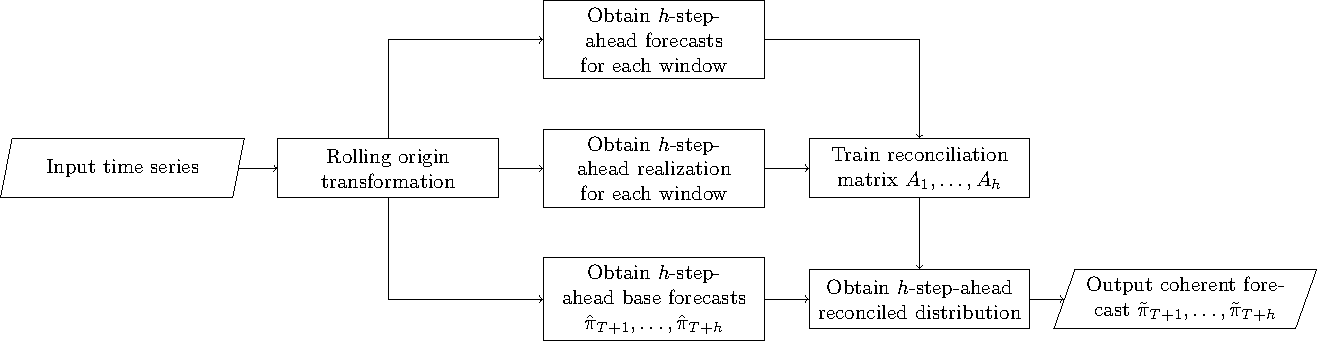
\includegraphics[width=\textwidth]{figures/DFR.pdf}
    \caption{\label{fig:dfr}Flowchart for the DFR algorithm.}
    \end{figure}


    \subsection{Stepwise discrete reconciliation}
    \label{sec:algorithm2}

    Although the so-called movement restriction reduces the dimension, the exponential growth of domain cardinalities still results in an exponential growth of the number of unknown parameters that need to be estimated.
    As a result, it is impossible to handle a high-dimensional hierarchy using the DFR algorithm alone.
    To address this issue, we propose a Stepwise Discrete Forecast Reconciliation (SDFR) algorithm that can overcome the curse of dimensionality.
    Instead of reconciling forecasts of all series at once,  SDFR
    decomposes a high-dimensional hierarchy into multiple two-level hierarchies with three nodes and reconciles these sub-hierarchies step by step using the DFR algorithm shown in \ref{sec:algorithm1}.
    This reduces the number of unknown parameters of each reconciliation process order $O(n^3)$.
    Given reasonable assumptions, we adjust the reconciled forecasts for these sub-hierarchies to construct joint forecasts for the entire hierarchy. As in the DFR algorithm, SDFR also consists of training and forecasting stages. The forecasting stage is shown in Algorithm \ref{alg:stepwise}, while training has a similar procedure.
    \begin{algorithm}[ht]
    \caption{\label{alg:stepwise}\textbf{S}tepwise \textbf{D}iscrete \textbf{F}orecast \textbf{R}econciliation (\textbf{SDFR})}
    \SetKwFunction{reconcile}{DFR$_i$}
    \SetKwFunction{bu}{BottomUp}
    \SetKwFunction{adjust}{Adjust}
    \SetKwFunction{construct}{ConstructJointDist}
    \SetKwInOut{Input}{Input}
    \SetKwInOut{Output}{Output}
    \Input{$\hat{\pi}_0,\dots,\hat{\pi}_k$}
    \For {$i=1,\dots,k-1$}{
      $\hat{\pi}_{\mathbf{S}_{k-i}} \leftarrow$ \bu($\hat\pi_{i+1},\dots,\hat\pi_k$)\;
      \uIf{ i = 1}{
        $\hat{\pi}_{\mathbf{S}_{k-i+1}} \leftarrow \hat\pi_0$ \;
      }
      \Else{$\hat{\pi}_{\mathbf{S}_{k-i+1}} \leftarrow \sum_{\mathbf{S}_{k-i+2}, y_{i-1}}\tilde{\bpi}(\mathbf{S}_{k-i+2}, y_{i-1}, \mathbf{S}_{k-i+1})$\;
      }

      $\tilde{\pi}(\mathbf{S}_{k-i+1}, y_i, \mathbf{S}_{k-i}) \leftarrow$ \reconcile{$\hat{\pi}_{\mathbf{S}_{k-i + 1}}, \hat\pi_{i}, \hat\pi_{\mathbf{S}_{k-i}}$}
    }

    \For {$i=2,\dots,k-1$} {
      $\tilde\pi^{1}_{\mathbf{S}_{k-i+1}} \leftarrow \sum_{\bY_{i-1}}\tilde{\bpi}(\bY_{i-1}, \mathbf{S}_{k-i+1})$ \;
      $\tilde\pi^{2}_{\mathbf{S}_{k-i+1}} \leftarrow \sum_{y_i,\mathbf{S}_{k-1}}\tilde{\bpi}(\mathbf{S}_{k-i+1}, y_i, \mathbf{S}_{k-i})$ \;
      $\tilde\pi'_{\mathbf{S}_{k-1+1}} \leftarrow \frac{1}{2} (\tilde\pi^{1}_{\mathbf{S}_{k-i+1}} + \tilde\pi^{2}_{\mathbf{S}_{k-i+1}}$) \;
      $\tilde{\bpi}'(\bY_{i-1}, \mathbf{S}_{k-i+1}) \leftarrow$ \adjust($\tilde{\bpi}(\bY_{i-1}, \mathbf{S}_{k-i+1}), \tilde{\pi}'_{\mathbf{S}_{k-i+1}})$ \;
      $\tilde{\bpi}'(\mathbf{S}_{k-i+1}, y_i, \mathbf{S}_{k-i}) \leftarrow$ \adjust($\tilde{\bpi}(\mathbf{S}_{k-i+1}, \mathbf{S}_{k-i+1}), y_i, \tilde{\pi}'_{\mathbf{S}_{k-i+1}})$ \;
      $\tilde{\bpi}(\bY_i, \mathbf{S}_{k-i}) \leftarrow$ \construct($\tilde{\bpi}'(\bY_{i-1}, \mathbf{S}_{k-i+1}), \tilde{\bpi}'(\mathbf{S}_{k-i+1}, y_i, \mathbf{S}_{k-i}) $)\;
    }
    \Output{$\tilde \bpi(\bY_k)$}

    \end{algorithm}

  Taking a hierarchy with one total series and $k~(k>3)$ bottom series as an example, Algorithm \ref{alg:stepwise} shows how independently generated base forecasts can be reconciled into coherent joint forecasts step-by-step when $k$ is large.
  Denote the total series as $y_0$ and bottom-level series as $y_1, \dots, y_k$.
  Denote the vector of first $i+1$ variables as $\mathbf{Y}_i$ and the sum of last $j$ variables as $\mathbf{S}_j$, i.e.,
  \[
    \bY_i = (y_0, \dots, y_i)', \quad \mathbf{S}_j = \sum_{l=k-j+1}^{k} y_l.
  \]
  In general, the hierarchy is split into $k-1$ three-node hierarchies.
  For each hierarchy $i$, one bottom series (the left node) corresponds to the node $i+1$ in the original hierarchy, i.e., $y_{i}$. The other bottom series (the right node) corresponds to $\mathbf{S}_{k-i}$, which is the sum of the remaining $k-i$ series; thus making $\mathbf{S}_{k-i+1}$ their total node.
  In the training stage, the reconciliation model \code{DFR}$_i$ is trained for this hierarchy.
  Base forecasts of the left node are obtained from input, while base forecasts of the right node are obtained using a bottom-up approach that will be discussed in Section~\ref{sec:bottomup}.
  The base forecasts for the total node are derived from the marginal distribution of that same node from the coherent distribution obtained in the previous step.
  One can obtain base forecasts for the right and total node by forecasting directly $\mathbf{S}_{j}, j=2,\dots,k-1$, which is applicable for cross-sectional hierarchies.
  However, in temporal hierarchies, forecasting $\mathbf{S}_{k-i+1}$ means forecasting temporal aggregation of partial time periods, introducing non-integer frequency problems and making it more challenging to capture time series dynamics.
  Our approach instead offers simple implementation with no extra expert intervention or modelling and can be applied to both cross-sectional and temporal hierarchies.

  During the forecasting stage, we first pass the base forecasts stepwise into these models to obtain $k-1$ coherent forecasts.
  Adjacent hierarchies share the same node (i.e., $\mathbf{S}_{k-i+1}$), but their marginal forecasts for the shared node (i.e., $\tilde\pi^{2}_{\mathbf{S}_{k-i+1}}$ and $\tilde\pi^{1}_{\mathbf{S}_{k-i+1}}$) are not identical because reconciliation generally changes input forecasts.
  We average these two marginal forecasts and pass their average into the \code{Adjust} algorithm, which adjusts the joint distributions from two adjacent steps to make their marginalisations of the shared node equivalent to the average.
  The two adjusted distributions are then passed into the \code{ConstructJointDist} algorithm to construct a new joint distribution.
  For space-saving purposes here, the \code{Adjust} and \code{ConstructJointDist} algorithms are shown in \ref{appendix:adjust}.

  Note that in our proposed algorithm, the result is sensitive to the order in which the bottom level series are combined. Consequently, we average results over different random orders of the bottom-level series; this reduces forecast uncertainty introduced by the \code{Adjust} and \code{ConstructJointDist} algorithms.
  When handling hierarchy with more aggregation levels, we can repeat the above procedure for each aggregated series either in a bottom-up or top-down manner. This means we reconcile the base forecasts of one level and use the reconciled forecasts as base children forecasts(bottom-up) or base parent forecasts (top-down) to reconcile the next level.



    \subsection{Probabilistic extensions of bottom-up and top-down methods for count series}

    Having extended the framework of forecast reconciliation to the discrete case, we can also define discrete analogues to the traditional top-down and bottom-up reconciliation methods. These will be used as benchmarks in our empirical examples. These methods require forecasts at a single level, which they then use to generate forecasts at other levels through disaggregation (top-down) or aggregation (bottom-up).
    We refer to these algorithms as Discrete Bottom-Up (DBU) and Discrete Top-Down (DTD) methods and both are special cases of our reconciliation framework. 
    
    \subsubsection*{\textbf{Discrete bottom-up}}
    \label{sec:bottomup}

    The discrete bottom-up method constructs a coherent distribution by assuming independent bottom-level forecasts.
    This method follows the same procedure as constructing base forecasts explained in Section~\ref{sec:algorithm1} except that the base forecasts of aggregated series are excluded.
    Using the three-variables example, $\tilde{\pi}_{(000)} = Pr(Y_1=0)\times Pr(Y_2=0)$.
    The linear reconciliation framework can also incorporate this method by marginalising out all aggregated time series from the incoherent base distribution, which yields \[
    \mathbf{A} = [\mathbf{I}_4, \quad \mathbf{I}_4, \quad \mathbf{I}_4 ].
    \]
    Note that the mean point forecasts obtained from this coherent distribution's marginal distribution are identical to those obtained by directly aggregating mean forecasts of bottom-level series.
    In other words, discrete bottom-up is compatible with the traditional bottom-up methods.

    Although it is possible to learn the dependence structure between bottom-level time series (e.g., empirical copulas used in \citealp{bentaiebHierarchicalProbabilisticForecasting2020}), we stick to the independence assumption due to its simplicity.

    \subsubsection*{\textbf{Discrete top-down}}

    The discrete top-down method extends the traditional top-down by proportionally disaggregating the probabilities of each point of the total series into all possible coherent points, using a ratio computed from historical occurrences.
    For example, if there are $40$ $(0, 1, 1)$ points and $60$ $(1, 0, 1) $ points observed in the three-variables scenario where $Pr(y_3) = 0.4$, the probabilities of possible coherent points would be calculated as follows: $\tilde \pi_{(011)} = 0.4\times 0.4$ and $\tilde \pi_{(101)} = 0.4\times 0.6$.
    This method can also be considered as a special case of Equation \eqref{eq:framework}, where
    \[
    \mathbf{A} = \left[\begin{matrix}
      1 & 1 & 1 & 1 & 0 & 0 & 0 & 0 & 0 & 0 & 0 & 0 \\
      0 & 0 & 0 & 0 & 0.4 & 0.4 & 0.4 & 0.4 & 0 & 0 & 0 & 0 \\
      0 & 0 & 0 & 0 & 0.6 & 0.6 & 0.6 & 0.6 & 0 & 0 & 0 & 0 \\
      0 & 0 & 0 & 0 & 0 & 0 & 0 & 0 & 1 & 1 & 1 & 1
    \end{matrix}\right].
    \]

\section{Simulation}
\label{sec:simulation}

To showcase the effectiveness of our proposed framework, we conduct two simulation experiments in distinct contexts: one for cross-sectional settings and another for temporal settings.

  \subsection{Cross-sectional hierarchy}
  \label{sec:cross-sectional_simu}
    \subsubsection{Simulation setup}
    This subsection considers the three-variables hierarchy depicted in Section~\ref{sec:example}.
    The binary count time series at the bottom level are generated based on underlying latent variables.
    We assume that these variables follow a bivariate VAR(1) process
    \[\mathbf{s}_t = \mathbf{\Phi}\mathbf{s}_{t-1}+\boldsymbol{\eta}_t,\]
    where
    \[
      \mathbf{\Phi} = \left[\begin{matrix}
        \alpha & 0 \\
        0 & \beta
      \end{matrix}\right], ~ \boldsymbol{\eta} \sim \mathcal{N}\left(\mathbf{0}, \left[\begin{matrix}
        0.1 & 0.05 \\
        0.05 & 0.1
      \end{matrix}\right]\right), ~ \mathbf{s}_{0} = \left[
        \begin{matrix}0 \\ 0\end{matrix}
      \right],
    \]
    and $\alpha$ and $\beta$ are uniformly generated from $[0.4, ~ 0.5]$ and $[0.3, ~ 0.5]$, respectively.
    This ensures the stationarity of the generated time series.
    The error term $\boldsymbol{\eta}$ implies a positive correlation between the two series and ensures a reasonable range of the latent state.
    Observations are transformed from the state series ($\mathbf{s}_{t} := [s_{1t}, s_{2t}]'$) using a sign function:
    \[
        Y_{it} = \mathbbm{1}(\sigma(s_{it}) > 0.5), ~ i\in\{1, 2\},\quad \sigma(s_{it}) = \frac{\exp(s_{it})}{1+\exp(s_{it})}.
    \]

    We produce and evaluate one-step-ahead forecasts in this experiment.
    For each binary series, we generate $480$ observations; the rolling origin strategy with $150$ observations used to train the base forecasting models is employed, yielding $330$ observations.
    The first $300$ observations are used to train the DFR model, while the remaining $30$ observations are used to test performance.

    The base probabilistic forecasts are obtained independently using the binomial AR(1) model~(\citealp{weissParameterEstimationBinomial2013}), which is suitable for count time series with a finite range.
    We evaluate the performance based on average Brier scores of the joint distribution of hierarchy and marginal distribution of each series on the $30$ test observations.


    We consider four benchmarks in this experiment and all other experiments in the rest of this paper, including base forecasts, discrete bottom-up, discrete top-down and empirical distribution. 
    The empirical distribution is a commonly used benchmark in the field of low-count time series forecasting.

    \subsubsection{Simulation results}
    The above procedure was repeated $1000$ times.
    Table~\ref{tab:sim_crosssectional_res_dist} summarises the average Brier Scores of the $1000$ samples, compared with four benchmarks.
    The best average performance of the four approaches is indicated by bold text in each row.
    DFR performs the best for both the total series and the hierarchy.
    % The discrete bottom-up method beats discrete top-down in both the total and bottom levels, indicating the inferiority of the base forecasts of the total series.
    Meanwhile, DFR shows considerable improvement in the accuracy of the total series, which implies its ability to mitigate the risk of model misspecification.
    Similar results were obtained from forecast reconciliation for continuous variables as well.
    Note that the Brier Score for the joint distribution of the base method is significantly larger than that of other methods, primarily because of its incoherency nature.

    We also performed MCB tests (\citealp{koningM3CompetitionStatistical2005}) at a 95\% confidence level to test the statistical significance of differences in accuracy among these approaches.
    This testing approach computes the mean ranks of the four approaches across the whole simulated dataset without imposing any distributional assumptions.
    Non-overlapping grey intervals indicate statistically significant differences between methods.
    As shown in Figure~\ref{fig:sim_temporal_mcb_prob}, DFR performs significantly better than all other approaches for total series and the hierarchy.
    Note that MCB tests for the bottom series are conducted on all samples at the bottom level.

    \begin{figure}
      \centering
      \label{fig:mcb_crosssectional}
      \caption{Average ranks and 95\% confidence intervals for the four approaches in the cross-sectional simulation. The overall ranks of the approaches in terms of Brier scores are shown to the right of their names.}
      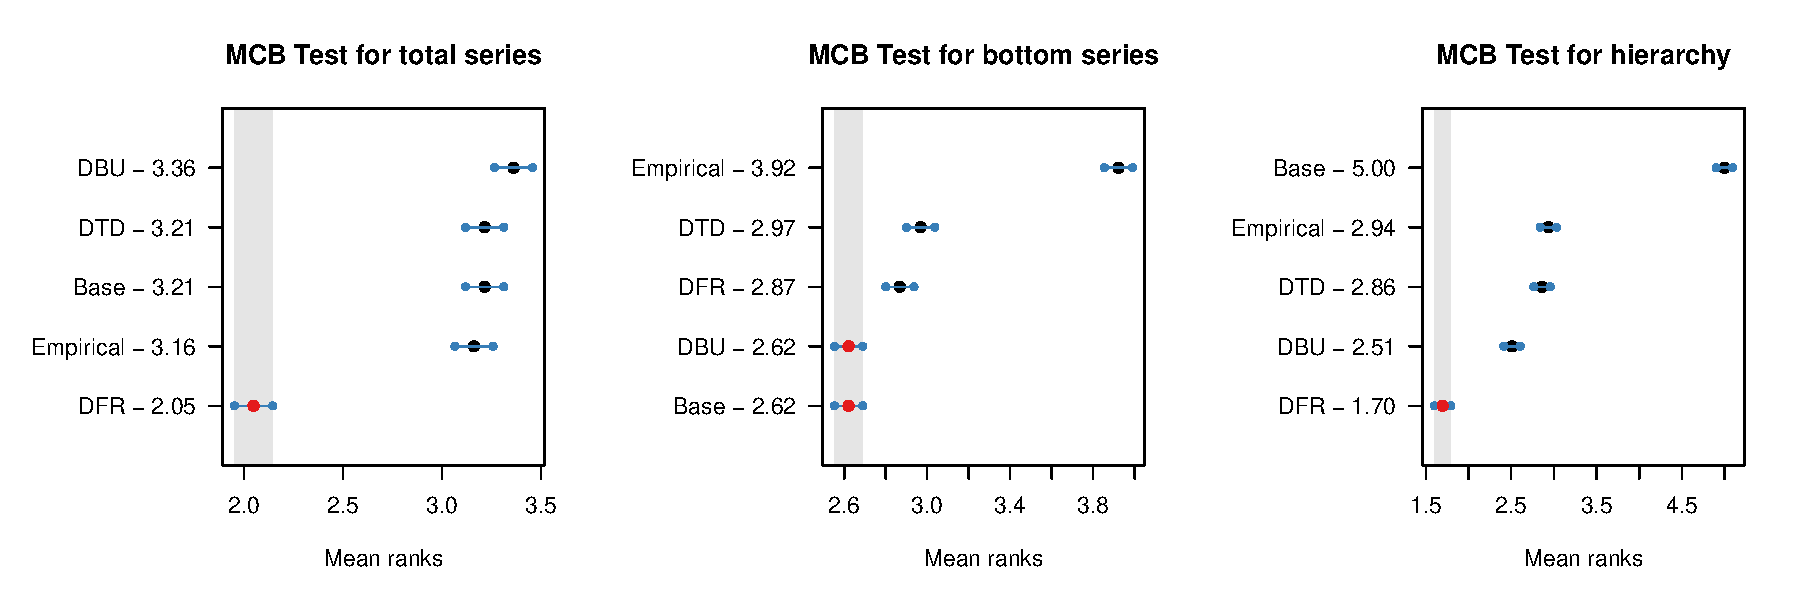
\includegraphics[width=\textwidth]{figures/sim_cross_mcb.pdf}
    \end{figure}


    \begin{table}
      \centering
      \caption{\label{tab:sim_crosssectional_res_dist} Probabilistic forecast performance summary for cross-sectional setting with Brier Score ($\times 10^{-2}$). Row-wise minimum values are displayed in \textbf{bold}.}
      \begin{tabular}{lccccc}
      \toprule
      % \multicolumn{5}{c}{Brier Score ($\times 10^{-2}$)}\\
      ~ & Base & DBU & DTD & DFR & Empirical \\ \midrule
      $Y_1$ & \textbf{46.52} & \textbf{46.52} & 47.25 & 46.78 & 50.41 \\ 
      $Y_2$ & \textbf{46.87} & \textbf{46.87} & 47.79 & 47.32 & 50.43 \\ 
      $Y_3$ & 67.07 & 67.13 & 67.07 & \textbf{64.57} & 67.15 \\ 
      Y & 88.65 & 71.23 & 72.00 & \textbf{69.60} & 72.9 \\ 
      \bottomrule
      \end{tabular}
    \end{table}


     \subsection{Temporal hierarchy}\label{sec:temporal_simu}
     We now consider a daily temporal scenario consisting of one total series and seven bottom-level series.
     This setting is frequently encountered in supply chain management, where daily and weekly forecasts are required to support operational decisions (\citealp{syntetosSupplyChainForecasting2016}).
     The bottom-level time series are restricted to values of 0 or 1.
     Despite this limitation, the hierarchy's domain remains extensive, making it difficult to estimate a complete reconciliation matrix with limited observations in practice.
     Therefore, we employ the stepwise reconciliation algorithm outlined in Section \ref{sec:algorithm2}.

     \subsubsection{Simulation setup}

     While intermittent series are characterised by fluctuating demand intervals and size at lower levels, they may exhibit seasonality and trend when temporally aggregated into higher levels (\Citealp{kourentzesElucidateStructureIntermittent2021}).
     Based on this understanding, we initially simulate weekly time series with a seasonal period of four, which are subsequently disaggregated into daily time series.

     Assuming that the weekly time series follows a Poisson distribution, we first simulate the conditional mean series utilising the autoregressive integrated moving average (ARIMA) process. This procedure is implemented with the \code{gratis} package \citep{gratis}
     for the \proglang{R} programming language. We set the seasonal period, number of autoregressive terms, difference order and seasonal difference order to $4$, $3$, $0$ and $0$, respectively. 
     Additional parameters are randomly produced by the package to ensure the diversity of the simulated series (\Citealp{kangGRATISGeneRAtingTIme2020}).
     Given that the domain of the weekly time series in our context is finite (i.e., $\leq 7$), we linearly map the generated conditional mean series into the range of $[2.5, 4.5]$.
     Subsequently, we simulate the Poisson distributed series based on the conditional mean series. Values exceeding $7$ are set to $7$.

     The weekly time series are then disaggregated into daily time series by randomly selecting days for which $Y=1$ and maintaining coherence.
     We first simulate seven probabilities based on seven independent Beta distributions $\textrm{B}(\alpha, \beta)$, corresponding to probabilities of $Y=1$ from Monday to Sunday.
     The values of the $w$ days with the highest probabilities are set to $1$, while others are set to $0$. Here, $w$ denotes the value of the corresponding weekly observation.
     $\beta$ is set to $4$ and $\alpha$ is set to $\alpha_i = i, i=1,\dots,7$, allowing for the probabilities of $Y=1$ to increase gradually from $i=1$ to $i=7$, suggesting potential seasonality.

     For each daily time series, $1003$ observations are generated, and the initial $100$ observations are discarded as warm-ups. Analogous to Section~\ref{sec:cross-sectional_simu}, we utilise the rolling origin strategy with a fixed look-back window size of $350$, yielding $547$ windows.
     For each rolling timestamp, the most recent $350$ observations are used as input to generate probabilistic forecasts for the following seven days.
     The initial $526$ samples are used to train the reconciliation model, and the final $21$ samples are to assess the forecasting performance.

     Base forecasts of daily time series are generated utilising an autoregressive logistic model.
     Specifically, for each origin, we construct an individual logistic model that employs the previous six observations and weekly dummy variables as regressors to predict the subsequent observation.
     To generate forecasts for the final seven days, at each step, we use the predicted value from the previous step as a regressor to predict the next step recursively.
     We implement the logistic regression model with the \code{glm} function in \proglang{R}.

     Base forecasts of weekly time series are generated using integer-valued GARCH $(\textrm{INGARCH})$ models (\Citealp{fokianosPoissonAutoregression2009}).
     Assuming that observations are Poisson distributed, the $\textrm{INGARCH}$ model utilises past observations and conditional mean to fit the conditional mean of current observation. The model $\textrm{INGARCH}(p, q)$ has the following form:
     \[
      \lambda_t = \beta_0 + \sum_{k=1}^p \beta_ky_{t-k} + \sum_{l=1}^q \alpha_l\lambda_{t-l}, 
     \] where $\beta_k, k=0,\dots,p$ and $\alpha_l, l=1,\dots,q$ are unknown parameters. $\lambda_t$ is the conditional mean at time $t$.
     For the sake of simplicity, we construct $\textrm{INGARCH}(3, 3)$ models for all weekly time series, which take the conditional mean and observations from the most recent three steps as regressors.
     We implement the $\textrm{INGARCH}$ model utilising the \code{tscount} package(\Citealp{liboschikTscountPackageAnalysis2017}) for \proglang{R}.
     Given the predicted mean of Poisson distribution within the forecast horizon, we add the probability of the series taking values greater than its maximum up to the probability of taking its maximum value.
     The base forecasts are then reconciled using the \textrm{SDFR} algorithm.


     \subsubsection{Simulation results}
     We repeated the simulation process $1000$ times.
     Table~\ref{tab:sim_temporal_res_dist} summarises the probabilistic forecast performance of the stepwise reconciliation model compared to four benchmarks.
     $Y_1,\dots,Y_7$ represent the daily series at the bottom level, while $Y_8$ denotes the weekly series at the total level.
     Although SDFR does not enhance forecast accuracies for all series, the results demonstrate a compromise between discrete top-down and discrete bottom-up methods.
     The inadequate performance exhibited by discrete top-down and empirical distribution models when applied to bottom-level series and the hierarchical might stem from their oversight of the autocorrelation embedded within the time series. 
     
     One intriguing observation is that the forecasting accuracy improves for $Y_4$ through $Y_7$.
     This could be attributed to the stepwise implementation of SDFR, which progresses from $Y_1$ to $Y_7$. The coherent forecasts of the previous series must be adjusted multiple times to construct the final joint distribution, thereby introducing uncertainty.
     Another explanation could be the effective utilisation of forecast combination, where the bottom-level series corresponding to the end of the week incorporates more forecasts than preceding ones.
     Surprisingly, the forecast accuracy of the total series does not exhibit significant deviation from base forecasts,  even though it is adjusted most frequently, showcasing the robustness of SDFR.
     It is crucial to note that the results could vary if the SDFR algorithm is implemented in a different step order.
     Additionally, the performance could be enhanced if we average multiple reconciled forecasts from various orderings.


     Figure~\ref{fig:sim_temporal_mcb_prob} displays the results of MCB tests to test the significance of differences in forecast performance among these approaches. Similar to the conclusions drawn from Table~\ref{tab:sim_temporal_res_dist}, SDFR significantly outperforms the other approaches in forecasting the bottom series and the hierarchy, while its forecasts for the total series do not deviate much from base forecasts.

     \begin{table}
     \centering
     \caption{\label{tab:sim_temporal_res_dist} Probabilistic forecast performance summary of temporal setting with Brier Score ($\times 10^{-2}$). Row-wise minimum values are displayed in \textbf{bold}.}
     \begin{tabular}{lccccc}
     \toprule
      & Base & DBU & DTD & SDFR & Empirical \\\midrule
      $Y_1$ & \textbf{40.78} & \textbf{40.78} & 49.40 & 40.95 & 49.79 \\ 
      $Y_2$ & \textbf{41.39} & \textbf{41.39} & 49.61 & 41.52 & 49.75 \\ 
      $Y_3$ & \textbf{42.06} & \textbf{42.06} & 49.86 & 42.07 & 49.73 \\ 
      $Y_4$ & 43.02 & 43.02 & 50.03 & \textbf{42.78} & 49.72 \\ 
      $Y_5$ & 43.56 & 43.56 & 50.22 & \textbf{43.09} & 49.73 \\ 
      $Y_6$ & 44.00 & 44.00 & 50.27 & \textbf{43.33} & 49.73 \\ 
      $Y_7$ & 44.31 & 44.31 & 50.28 & \textbf{43.92} & 49.78 \\ 
      $Y_8$ & 82.58 & 83.48 & 82.58 & 83.11 & \textbf{82.55} \\ 
      $Y$ & 99.54 & 97.77 & 99.36 & \textbf{97.74} & 99.12 \\ 
     \bottomrule
     \end{tabular}
     \end{table}


     \begin{figure}
       \caption{\label{fig:sim_temporal_mcb_prob}Average ranks and 95\% confidence intervals for the four approaches in the temporal simulation. The overall ranks of the approaches in terms of Brier scores are shown to the right of their names.}
       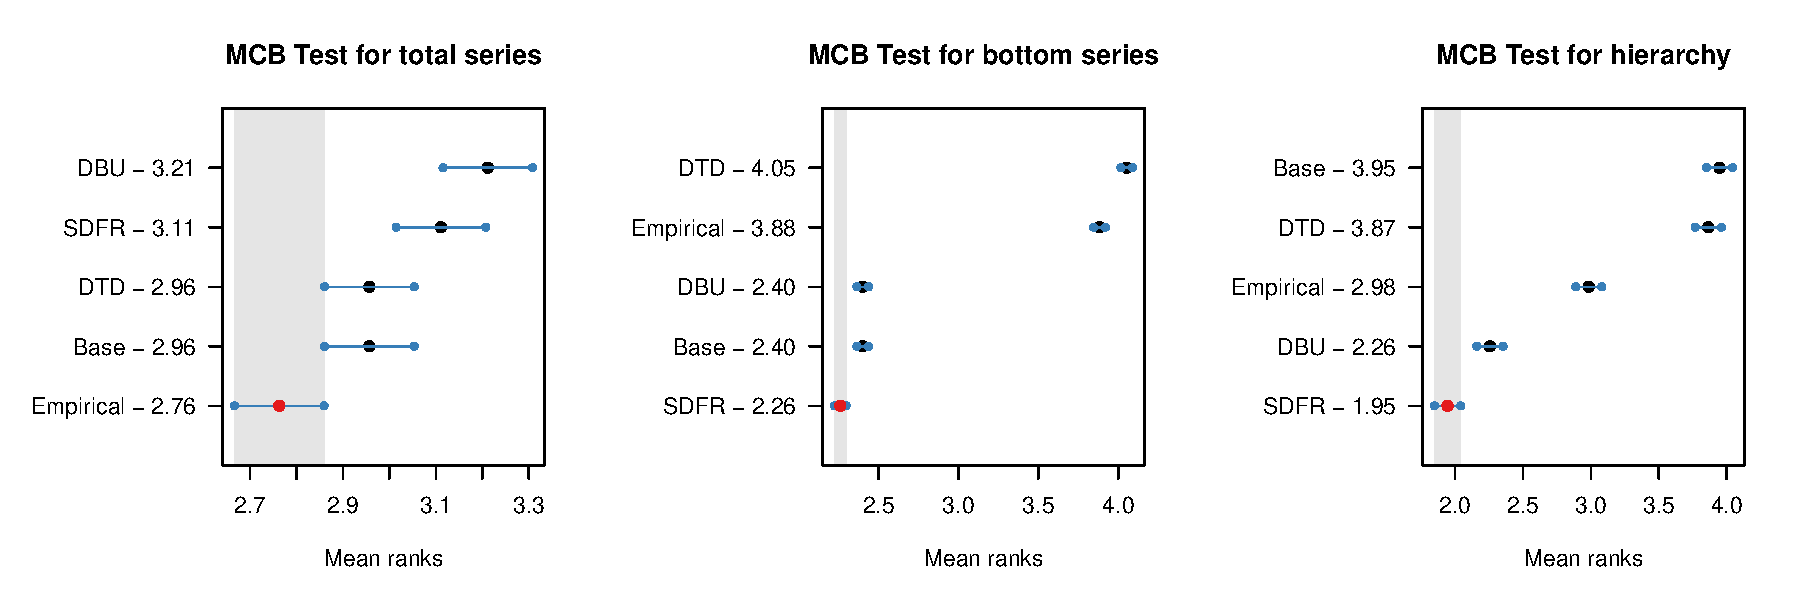
\includegraphics[width=\textwidth]{figures/temporal_mcb.pdf}
     \end{figure}

     \section{Empirical study}
     \label{sec:application}
     This section uses the proposed DFR algorithm to forecast two publicly available real-world datasets.
     Section~\ref{sec:application_crime} concentrates on temporal hierarchy and forecasts the number of criminal offences in Washington D.C.
     Meanwhile, Section~\ref{sec:M5} constructs and forecasts cross-sectional count hierarchical time series in the M5 dataset.

     \subsection{Application: forecasting crime in Washington D.C.}
     \label{sec:application_crime}

     Forecasting crime numbers in a specific area is vital for managing public safety and police resources.
     However, forecasting becomes more challenging when dealing with smaller areas with sparse crime numbers.
     In this subsection, we apply the proposed DFR algorithm to predict the number of offence crimes in census tracts located in Washington, D.C.
     The original dataset\footnote{The dataset can be downloaded from \url{https://crimecards.dc.gov/}.} contains all reported crimes from 2014 to 2022 in Washington D.C., which have been aggregated into weekly time series according to location and crime type.
     Considering the domain of the number of crimes, we perform experiments on all time series whose location type is a census tract and crime type is offence.
     As a result, we obtain $231$ weekly time series; each representing the number of offence crimes committed within one census tract.

     The crime numbers time series are potentially autocorrelated (\citealp{aldor-noimanSpatioTemporalLowCount2013}).
     Our objective is to generate coherent probabilistic forecasts for the next four weeks.
     To achieve this, we construct two-level temporal hierarchies that consist of weekly (bottom level) and four-weekly (total level) frequencies and develop an individual DFR model for each time series.
     Additionally, we restrict the maximum value (i.e., the domain of the bottom level in the DFR model) of the weekly time series as follows: if the largest observation is $1$, then its domain is set to $[0, 1]$.
     Otherwise, it is set to $[0, 1, 2]$.
     Any observation exceeding $2$ is truncated at $2$.
     Notably, less than one percent of observations surpass $2$, so these adjustments have a negligible impact on the final results.

     We adopt the rolling origin strategy to train and evaluate our discrete reconciliation model.
     Initially, we produce four-step-ahead probabilistic forecasts using INGARCH(3, 4) from a time series of $53$ weeks.
     Subsequently, we augment the training data by one week and produce new probabilistic forecasts.
     At each step, to obtain the probabilistic forecasts for the total level, we first aggregate the weekly series into four-weekly time series and then use INGARCH(2, 2) to produce one-step-ahead forecasts.
     We only use windows with forecast horizons starting before $2022$ as training samples; all remaining windows are used for performance evaluation purposes.
     We repeat the above procedure for each census tract, resulting in a total of $3696$ samples ($231$ census tracts multiplied by $16$ test samples per census tract).
     These reconciled forecasts are then used to evaluate forecasting performance.

     We calculate Brier Scores for each sample at the total level, the bottom level and the entire hierarchy.
     Table~\ref{tab:crime_bs} summarises the mean Brier Score of the $3696$ samples.
     We also perform MCB Test to indicate the significance of the difference, with results shown in Figure~\ref{fig:application_crime}.

     \begin{table}[h]
       \centering
       \caption{\label{tab:crime_bs}Summarised Brier Score ($\times 10^{-2}$) of test samples in crime forecasting application. Row-wise minimum values are displayed in \textbf{bold}.}
       \begin{tabular}{cccccc}
       \toprule
       ~ & Base & DBU & DTD & DFR & Empirical \\\midrule 
       Total & 58.36 & \textbf{58.02} & 58.36 & 58.09 & 59.12 \\ 
       Bottom & 34.34 & 34.34 & 34.73 & \textbf{34.25} & 34.54 \\ 
       Hierarchy & 73.73 & \textbf{67.75} & 68.18 & {67.85} & 68.69 \\ 
       \bottomrule
       \end{tabular}
       \end{table}

     \begin{figure}[h]
       \caption{\label{fig:application_crime}Average ranks and 95\% confidence intervals for the five approaches in the crime forecasting application. The overall ranks of the approaches in terms of Brier scores are shown to the right of their names.}
       \centering
       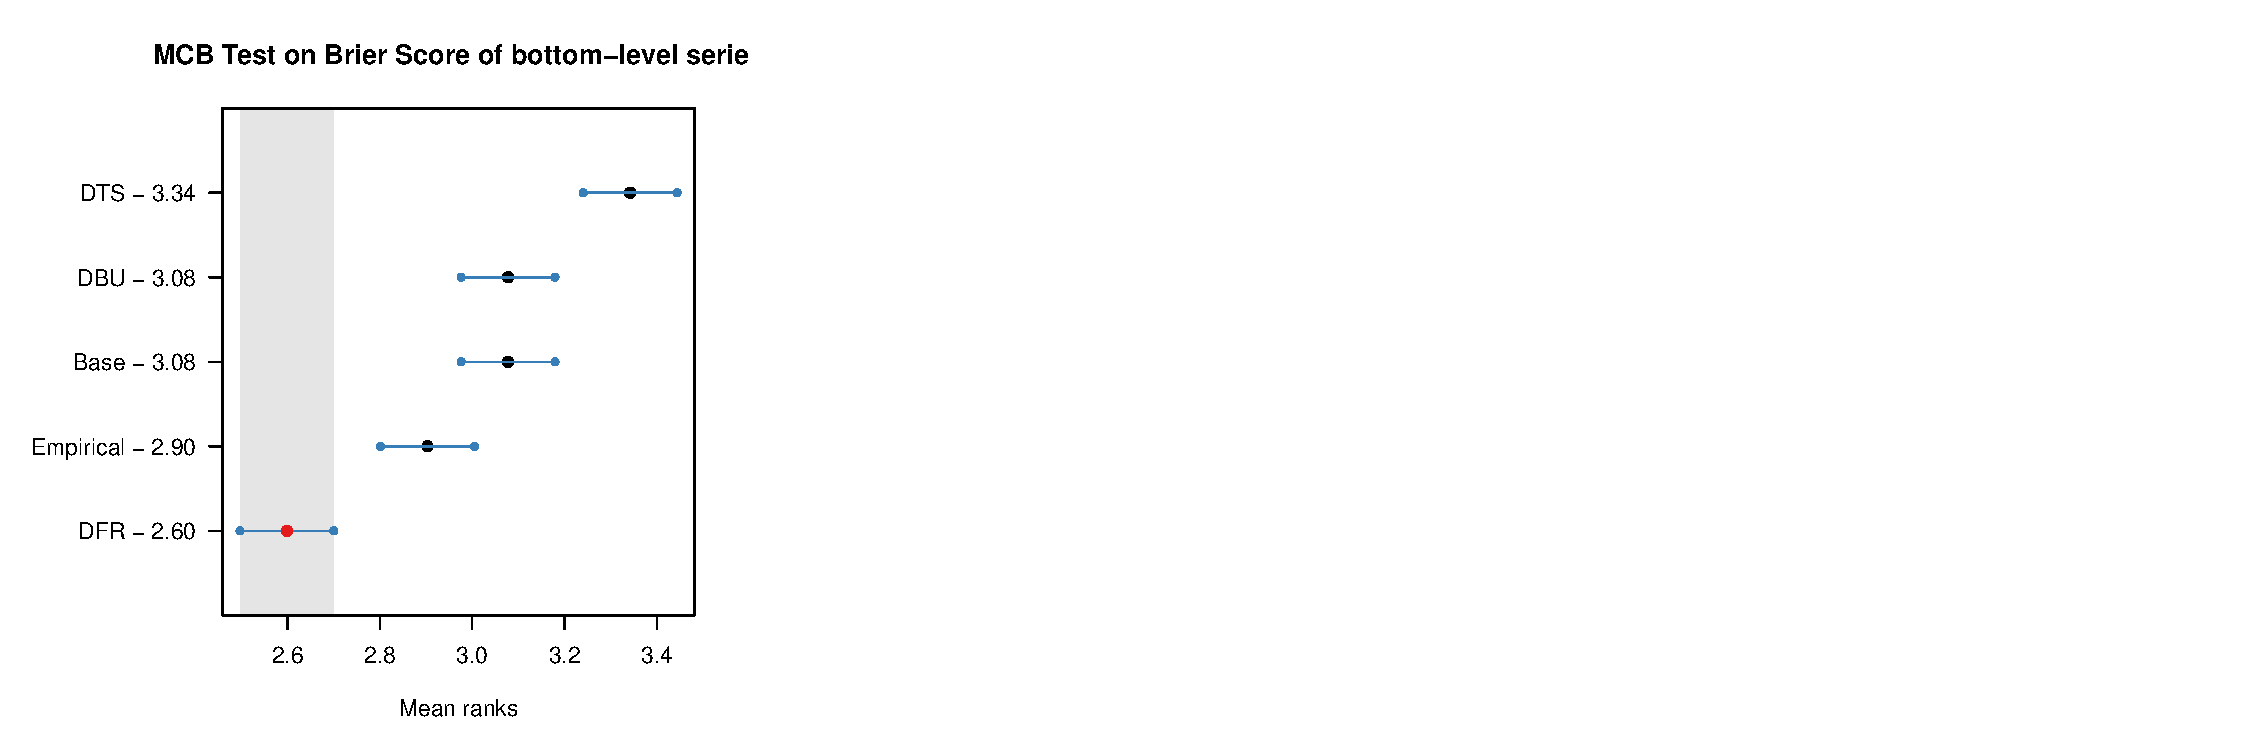
\includegraphics[width=\textwidth]{figures/dc_crime_mcb.pdf}
     \end{figure}


     In Table~\ref{tab:crime_bs},  although on average, the left panel shows that discrete bottom-up performs slightly better than DFR for both total level and whole hierarchy, DFR outperforms all other approaches in terms of average ranks. This indicates that DFR not only produces coherent forecasts but also improves forecasting accuracy. The most significant improvement occurs at the bottom level. Besides, the discrete bottom-up performs better than other methods, including the discrete top-down method, which suggests inferiority in total-level forecasts. The MCB test plots in Figure~\ref{fig:application_crime} demonstrate a statistical difference between DFR and other methods for bottom-level series. These findings imply that DFR is more effective than other approaches for more HTSs.

     \subsection{Application: forecasting intermittent demand in M5 dataset}
     \label{sec:M5}

     Intermittent time series are commonly observed in the modern database systems, where finer and finer granularity of data in hierarchies are collected. 
     Such time series are prevalent in the fields of inventory and supply chain management, supporting daily store replenishment, transportation plans, after-sales services and other applications(\citealp{babaiDemandForecastingSupply2022}).
     Coherent predictive distributions are critical for these fine-granularity hierarchies. 
     In this subsection, we apply the proposed SDFR algorithm to a subset of the M5 (\citealp{makridakisM5AccuracyCompetition2022}) dataset, which comprises $3049$ units of products sold by Walmart at ten stores located in three states in the USA from January 29, 2011 to May 23, 2016 (1941 days).
     
    We construct a cross-sectional State-Store hierarchy for single unit of product, where total series represents sales of the unit sold at a specific state, while bottom series represent sales of the unit sold at all stores at that state. 
    In order to restrict our attention to low-count intermittent time series, we exclude the hierarchies whose maximum sale of bottom series is greater than $4$. 
    In this experiment, we consider one-step-ahead forecast and employ the rolling origin strategy. The starting window size is chosen so that totally $730$ samples are produced, with the last $28$ samples are used for evaluation.
    Hierarchies that do not contain enough observations are also excluded.
    Finally, we obtain $665$ hierarchies to evaluate the performance of different approaches. 
    The base forecasts are produced using the model that combines SBA (\citealp{syntetosAccuracyIntermittentDemand2005}) forecasting method for intermittent demand and negative binomial distribution proposed in \cite{kolassaEvaluatingPredictiveCount2016}.

    Table~\ref{tab:M5} presents the accuracy of benchmarks and SDFR in terms of average Brier Score across $665$ hierarchies. The corresponding MCB test is displayed in Figure~\ref{fig:application_M5}. SDFR significantly outperforms the discrete top-down method and base forecasts across all levels. While it fails to outperform discrete bottom-up or empirical distribution on single level, it performs best in terms of brier score of the hierarchy. 
    Interestingly, the empirical distribution shows a competitive accuracy in this experiment. 
    One of the possible reason is that the time series in this application shows weak auto-correlation, making time series model offer less benefits.
    However, our SDFR model still improves the accuracy of the whole hierarchy compared to benchmarks in such circumstances.

    \begin{table}
        \centering
        \begin{tabular}{llllll}\toprule
            ~ & Base & DBU & DTD & SDFR & Empirical \\ \midrule
            Total & 50.86 & 50.57 & 50.86 & \textbf{50.34} & 50.35 \\ 
            Bottom & 23.97 & 23.97 & 23.90 & 23.83 & \textbf{23.82} \\ 
            Hierarchy & 62.74 & 55.87 & 56.02 & \textbf{55.63} & 55.64 \\ \bottomrule
        \end{tabular}
        \caption{\label{tab:M5}Summarised Brier Score ($\times 10^{-2}$) of test samples in M5 forecasting application. Row-wise minimum values are displayed in \textbf{bold}.}
    \end{table}


    \begin{figure}[h]
      \caption{\label{fig:application_M5}Average ranks and 95\% confidence intervals for the five approaches in the M5 application. The overall ranks of the approaches in terms of average Brier scores are shown to the right of their names.}
      \centering
      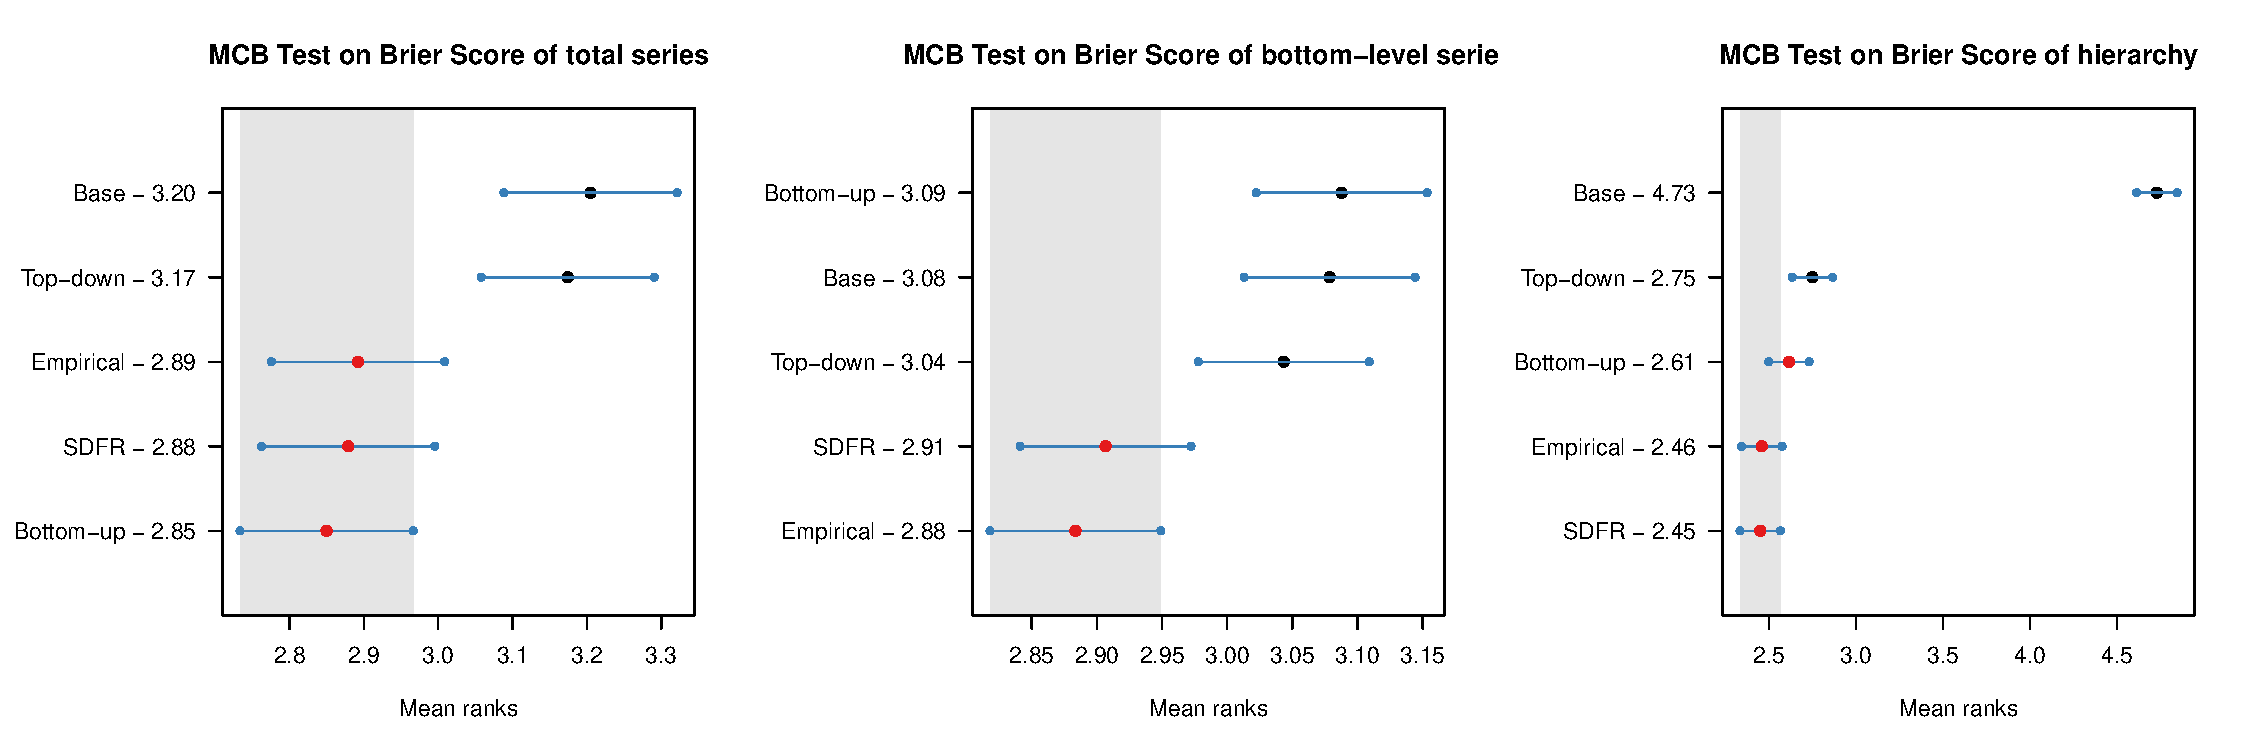
\includegraphics[width=\textwidth]{figures/M5_mcb.pdf}
    \end{figure}

     \section{Discussion}
     \label{sec:discussion}



     Distributional forecasts are becoming increasingly important in both academic and industry settings for operational research. In the context of hierarchical forecasting, \cite{kolassaWeWantCoherent2022} suggests shifting focus from coherent point forecasts to coherent probabilistic forecasts.
     The proposed discrete reconciliation framework can generate coherent distributional forecasts for discrete-valued HTS.
     Summary statistics such as median, mean, and quantiles can be derived from the marginal distribution obtained from the distributional forecasts.
     It is worth noting that mean point forecasts obtained in this way are also coherent in terms of aggregation.
     %Moreover, our methods offer precise distributions instead of relying on empirical distribution derived from sampling as seen in previous studies (e.g., \citealp{jeonProbabilisticForecastReconciliation2019,coraniProbabilisticReconciliationCount2022}).

     This paper focuses on linear reconciliation, achieved by multiplying the base incoherent probability vector with a reconciliation matrix.
     From a machine learning perspective, this procedure can be viewed as a classification problem with an $r$ dimensional output representing class probabilities and a $q$-dimensional input. Machine learning models, such as specifically designed neural networks, can be utilised to solve this problem.
     When thousands of time series need to forecast, cross-learning techniques can be employed to construct a global non-linear reconciliation model. This poses an interesting avenue for future research.

     One limitation of the proposed DFR algorithm is that it can not be easily applied to a large hierarchy, which requires more observations and computational resources due to the curse of dimensionality.
     While the SDFR algorithm mitigates this problem, it also introduces additional uncertainty.
     In order to shed more light on how the curse of dimensionality affects the computation and understand the capacity of the proposed approaches, we summarise the number of series, the number of parameters and the estimated single-run computational time for training the reconciliation model in our experiments. 
     The results are shown in Table~\ref{tab:time}. 
     Note that we only report values of the largest hierarchy due to varying hierarchies in empirical studies. 
     Computational time were evaluated on a machine equipped with a Microsoft Windows 10 system, an Intel Core i7-8700 processor clocked at 3.20GHz, providing six cores, and 16GB of memory.
     We suggest applying the proposed algorithm to small to moderate-sized hierarchies that have similar-size domains in our experiments. When applying to large hierarchies, the bottom-level series should be low-count, such as binary. For larger hierarchies, the top-level series are likely to be more easily modelled as continuous. Reconciliation of hierarchies with both discrete and continuous variables is a problem we leave to future research.

     \begin{table}
       \centering
       \resizebox{\textwidth}{!}{
       \begin{tabular}{lcccc}
        \toprule
        & Section~\ref{sec:cross-sectional_simu} & Section~\ref{sec:temporal_simu} & Section~\ref{sec:application_crime} & Section~\ref{sec:M5}\\ \midrule
        Number of bottom-level series & 2 & 7 & 4 & 4\\
        Maximum of bottom-level series & 1 & 1 & 2 & 4\\
        Cardinality of coherent domain & 4 & 128 & 81 & 625\\
        Cardinality of incoherent domain & 12 & 1024 & 729 & 10625 \\
        Number of parameters & 22 & 1312 & 9342 & 25420 \\ 
        Algorithm & DFR & SDFR & DFR & SDFR \\
        Computational time (seconds) & 0.1 & 1.6 & 311 & 1558\\ \bottomrule
       \end{tabular}}
       \caption{\label{tab:time} Reconciliation model size and computational time (in seconds) in the four experiments implemented in different sections.}
     \end{table}

     In our experiments, we have observed that the accuracy of some series' base forecasts is not ideal.
     We attribute this to three reasons. Firstly, it is challenging to forecast low count time series with excess zeros accurately.
     Secondly, we have not used state-of-the-art forecasting methods for such time series as proposed by \cite{berryBayesianForecastingMany2020a} and \cite{weissEfficientAccountingEstimation2022}.
     Thirdly, the parameters of the employed models are not optimally estimated.
     To improve performance in future work, we suggest using more modern forecasting methods and carefully selecting both models and the corresponding parameters.





     \section{Conclusion}
     \label{sec:conclusion}

     This paper develops a novel forecast reconciliation framework for count hierarchical time series.
     The framework involves assigning probabilities from incoherent points to coherent points, similar to the mapping approach for continuous time series.
     We further propose a linear reconciliation algorithm that minimises the penalised brier score of reconciled probabilistic forecasts.
     To address the exponential growth of the domain, we introduce a stepwise discrete reconciliation algorithm by breaking down a large hierarchy into smaller ones.
     We also propose probabilistic extensions of traditional top-down and bottom-up methods for count time series.

     Our DFR and SDFR algorithms produce coherent probabilistic forecasts and improve forecast accuracy.
     We demonstrate this through simulation experiments on cross-sectional and temporal hierarchies, where our algorithms outperform discrete top-down and discrete bottom-up approaches. Additionally, we apply the DFR algorithm to forecast crime numbers in Washington D.C. and sales of product units in the M5 dataset with promising results.
     The results indicate the potential of the proposed algorithms to be applied in reality.

     One key factor contributing to our strong results is the utilisation of forecast combinations.
     Similar to reconciliation approaches for continuous variables, our framework combines forecasts and the information used to produce forecasts at different levels.
     Also important is that our models train the reconciliation weights using out-of-sample forecasts generated by the rolling origin strategy, leading to robust results.


     While this work provides an explanatory attempt at discrete hierarchical time series forecasting, future research should focus more on real-world management problems associated with discrete cases. Count hierarchical time series forecasting remains an open issue that requires further attention from researchers in this area.

\section*{Acknowledgments}

Yanfei Kang is supported by the National Natural Science Foundation of China (No. 72171011). This research was supported by international joint doctoral
education fund of Beihang University and the high-performance computing (HPC) resources at Beihang University.


\begingroup
\setstretch{1.15}
\bibliographystyle{agsm}
\bibliography{references.bib}
\endgroup

\newpage

\appendix

\section{Algorithms}
\label{appendix:adjust}

The \code{Adjust} algorithm is used to adjust an existing multivariate joint distribution to make its marginalisation over one of the variables equal to that given by a reconciled distribution is a single step of the stepwise procedure.

\begin{algorithm}[H]
  \label{alg:adjust}
  \caption{\code{Adjust}}
  \SetKwInOut{Input}{Input}
  \SetKwInOut{Output}{Output}
  \Input{$\bpi(y_0,y_1,\dots,y_i), \tilde\pi_i, y_i \in \{0,1,\dots,k_i\}$}

  $\bpi(y_0,\dots,y_{i-1}) = \sum_{y_i}\bpi(y_0,\dots,y_i)$\;
  $\pi_i = \sum_{y_0,\dots,y_{i-1}}\bpi(y_0,\dots,y_i)$ \;
  \For { $j = 0,\dots,k_i$} {
    $\bpi'(y_0,\dots,y_{i-1}, y_i=j) = \bpi(y_0,\dots,y_{i-1}) \times \frac{\tilde\pi_i}{\pi_i}$ \;
  }

  \Output{$\bpi'(y_0,\dots,y_i)$}

 \end{algorithm}


 The \code{ConstructJointDist} algorithm constructs a new joint construct given two joint distributions.
 Consider variables $y_1, ~ \bY_2, ~ y_3, ~ y_4, ~ \bY_5$, where $\bY_2$ and $\bY_5$ are vectors and $y_1, ~ y_3, ~ y_4$ are scalars.
 They have the following relations.
 \[
  y_1 = |\bY_2|_1 + y_3, \quad y_3 = y_4 + |\bY_5|_1,
 \]
 where $|\cdot|_1$ represents the sum of all the variables in the vector.
 The given distributions are $\bpi(y_1, ~ \bY_2, ~ y_3)$ and $\bpi(y_3, ~ y_4, ~ \bY_5)$.
 The marginal distributions of $y_3$ derived from the two distributions are the same, i.e.,
 \[
  \sum_{y_3} \bpi(y_1, ~ \bY_2, ~ y_3) = \sum_{y_3}\bpi(y_3, ~ y_4, ~ \bY_5)
\]
 Assuming the joint distribution of $y_1$ and $\bY_2$ is independent of the joint distribution of $y_4$ and $\bY_5$ given $y_3$, we can obtain the probability of one point in the new joint distribution using the following equation: \[
   \begin{aligned}
  &\text{Pr}(y_1=a_1, ~ \bY_2=\mathbf{a}_2, ~ y_4=a_4, \bY_5 = \mathbf{a}_5) =\\ &\text{Pr} (y_1=a_1, ~ \bY_2=\mathbf{a}_2, ~ y_3=a_3) \times \text{Pr}(y_4=y_4, ~ \bY_5=y_5|y_3=a_3).
   \end{aligned}
 \]
 The equation constructs the joint distribution of $y_1, \bY_2, y_4, \bY_5$ by eliminating the shared variable $y_3$ of the two distributions.


\end{document}